%# -*- coding: utf-8-unix -*-
%%==================================================
%% chapter03.tex for SJTU Bachelor Thesis
%%==================================================

%\bibliographystyle{sjtu2}%[此处用于每章都生产参考文献]
\chapter{5G Cloud RAN中的负载均衡}
\label{chap:LB}
\section{无线移动通信系统基站的演进}
在第一代与第二代无线移动通信中,蜂窝网络(cellular),或无线电接入网(Radio Access Networks,缩写RAN),是由相互独立的基站组成的,每个基站配有电力、备用电源、空调系统、环境监测、回程链路等其他支持设施。每个基站内部含有射频信号发射单元,射频信号通过电缆从地面机柜传输至位于高处的基站天线。为了降低射频信号在电缆上的传输损耗,第三代移动通信采用了分布式基站系统。分布式基站将射频拉远单元(Remote Radio Head,缩写RRH)与基带信号单元(Baseband Unit,缩写BBU)分离,使RRH可以直接部署在基站塔顶距离天线很近的地方,并通过光纤的连接使两者间的距离变大(可达几百米或几千米)而损耗减小。建立在分布式基站架构的基础上,Cloud RAN为无线接入网引入了云技术,使很多BBU集中到一个BBU池。通过应用数据中心网络技术,Cloud RAN能够在BBU池中的BBU之间建立低功耗、高可靠、低延迟、高带宽的连接。它应用了开放的平台与实时虚拟化技术以实现动态共享的资源分配并支持多厂商、多种技术并存的环境。在这种技术架构下,由于BBU池覆盖的范围比原来的一个基站所能覆盖的范围大得多(即一个用户从一个RRH切换到另一个RRH时,他前后连接的两个BBU在同一个BBU池中)\cite{ran2015optimal},蜂窝系统中流量分布不均匀的问题可以通过在BBU池中部署灵活的、动态自适应的负载均衡算法得以解决。
\begin{figure}[h]
    \centering
    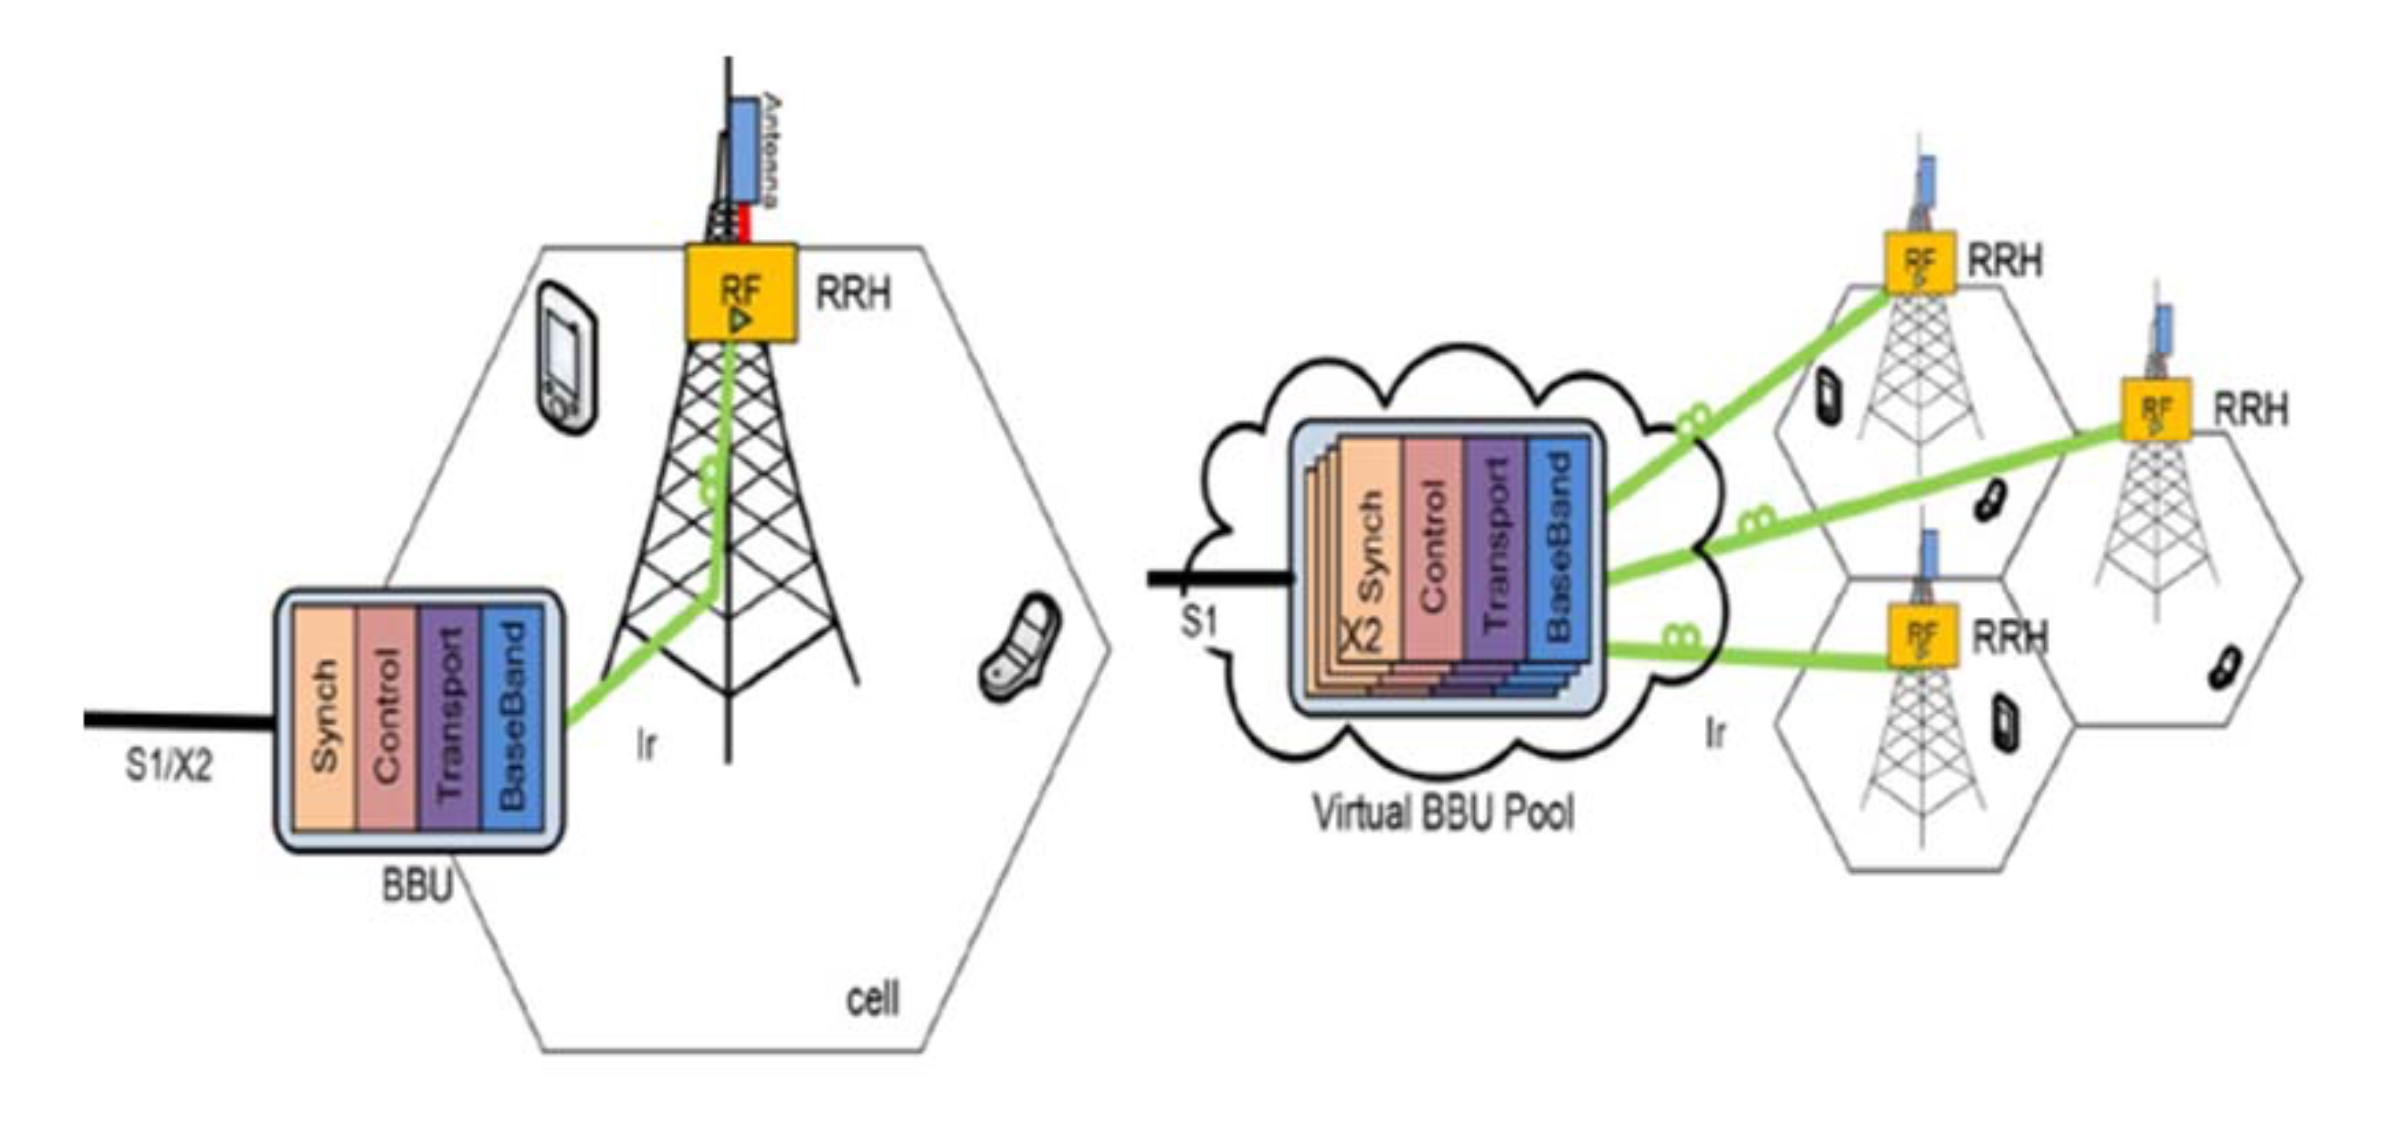
\includegraphics[height=4cm]{figure/CRAN.png}
    \caption{RAN(左)与Cloud RAN(右) \cite{tsai2017load}}
    \label{fig:CRAN}
\end{figure}
\section{5G时代的数据中心网络}
近年来,随着越来越多的企业和组织将其服务转向云端、云服务的需求日益增长,人们建立了很多规模庞大的数据中心。数据中心的大量服务器通过如Fat-Tree\cite{alfares2008fattree}、VL2\cite{greenberg2009vl2}、CamCube\cite{costa2012camcube}、DCell\cite{guo2008dcell}、BCube\cite{guo2009bcube}等可横向拓展的模型连接在一起,为云服务提供大量的计算资源。
\subsection{网络架构}
按网络架构的不同,数据中心可分为以交换机为中心、以服务器为中心和混合型三种架构。在以交换机为中心的架构中,交换机被用于提供服务器之间的多条通路连接以及数据包的转发;在以服务器为中心的架构中,服务器既提供计算功能还扮演着交换机的角色与其他服务器相连;混合型架构使用服务器与交换机共同实现数据的转发、并通常在服务器间提供多条不等长的路径。下面我们对每种架构举例说明:
\begin{itemize}
    \item \textbf{Fat-Tree}:Fat-Tree是一种以交换机为中心的多层结构,其拓扑从下到上分为三层:edge,aggregation和core。如图\ref{fig:fat-tree}所示,对于一个$k$叉树 ($k$-ary),Fat-Tree共包含$k$个pod,每个pod有两层交换机,每层有$\frac{k}{2}$个。每个交换机共有$k$个端口。在edge层,交换机的$\frac{k}{2}$个端口连接着$\frac{k}{2}$台服务器,剩余的$\frac{k}{2}$个端口连接aggregation层的交换机。在core层共有$\frac{k^2}{4}$个核心交换机,每个核心交换机有一个端口连接着$k$个pod中的一个。这种架构能够极大地减少部署交换机的开销,但也会导致较多的互连开销。
    \begin{figure}[h]
    \centering
    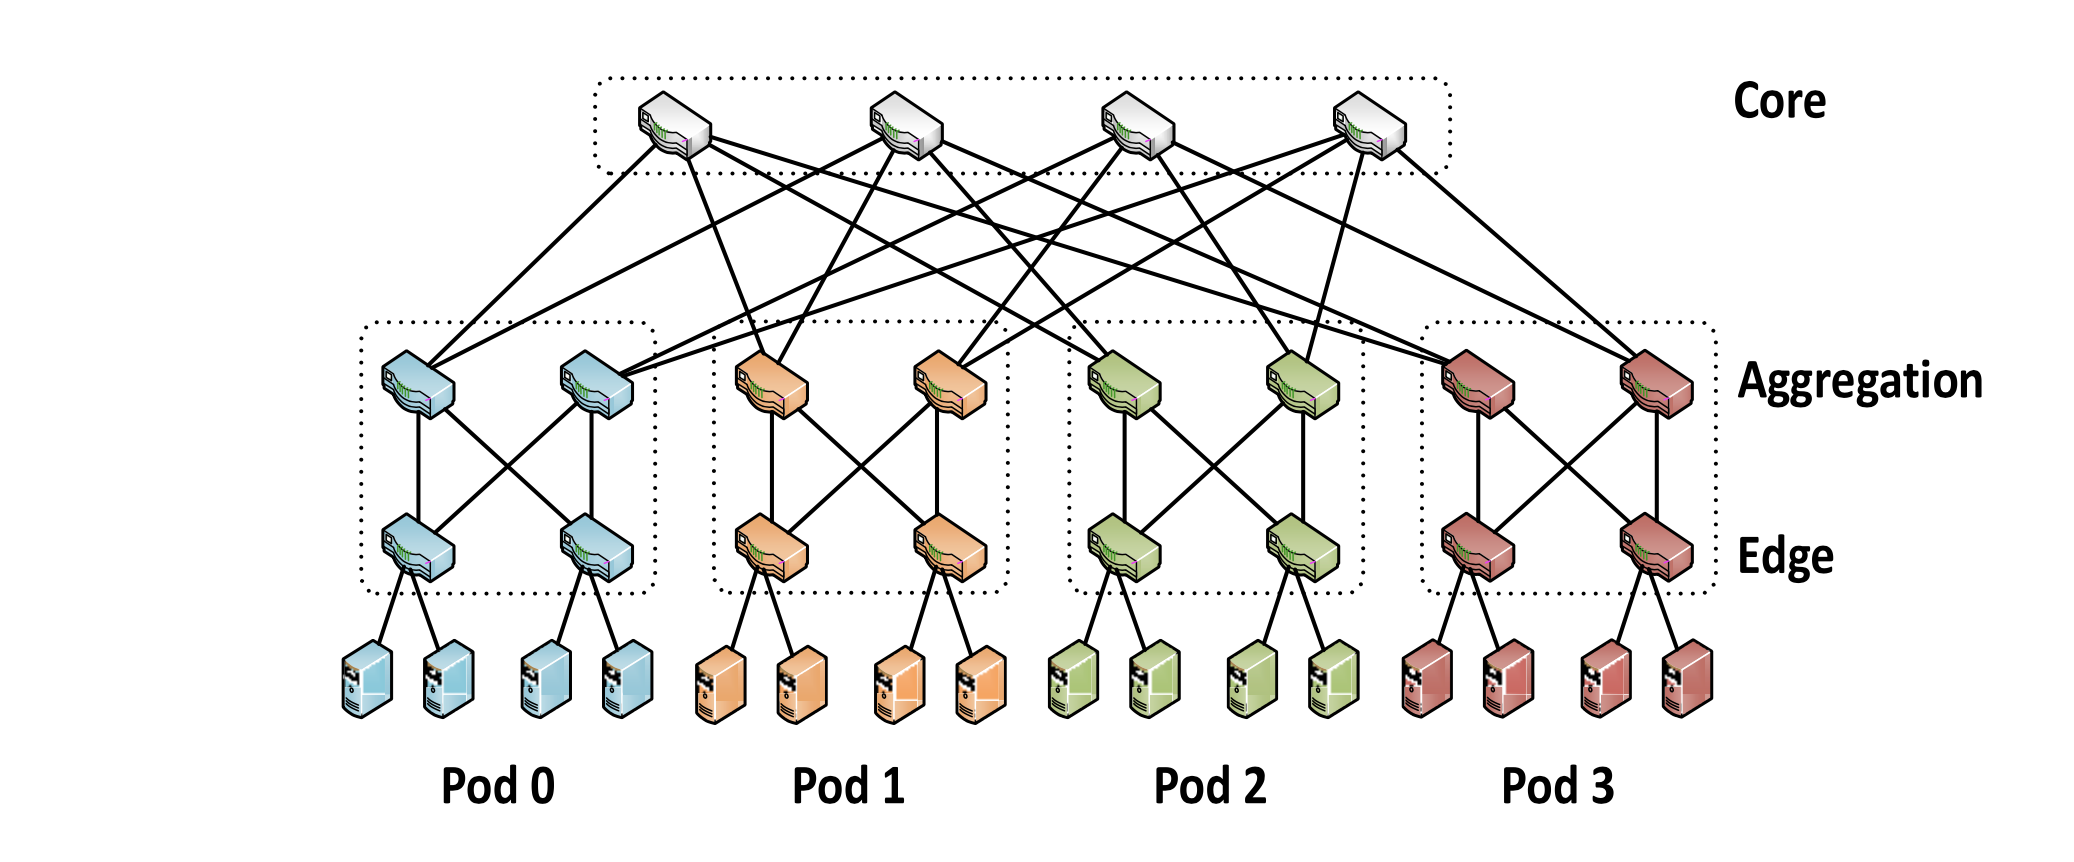
\includegraphics[height=4.5cm]{figure/fat-tree.png}
    \caption{Fat-Tree架构 (图中为$k$ = 4的情形) \cite{alfares2008fattree}}
    \label{fig:fat-tree}
    \end{figure}
    
    \item \textbf{CamCube}:CamCube是一种以服务器为中心的空间网状结构。图\ref{fig:camcube}展示的是含有27个服务器的3D-Torus结构。P. Costa在论文中提出了一种基于键(key)的网络,通过使用CamCube的API,能够充分利用空间网格结构的优越性,节省交换机和路由器的开销。同时由于服务器的散热开销小于交换机,这种结构比较节能。CamCube的主要缺点是对于非键值的应用,数据转发路径可能会很长,路由算法的复杂度可能会很高\cite{wang2014rethinking}。
    \begin{figure}[h]
    \centering
    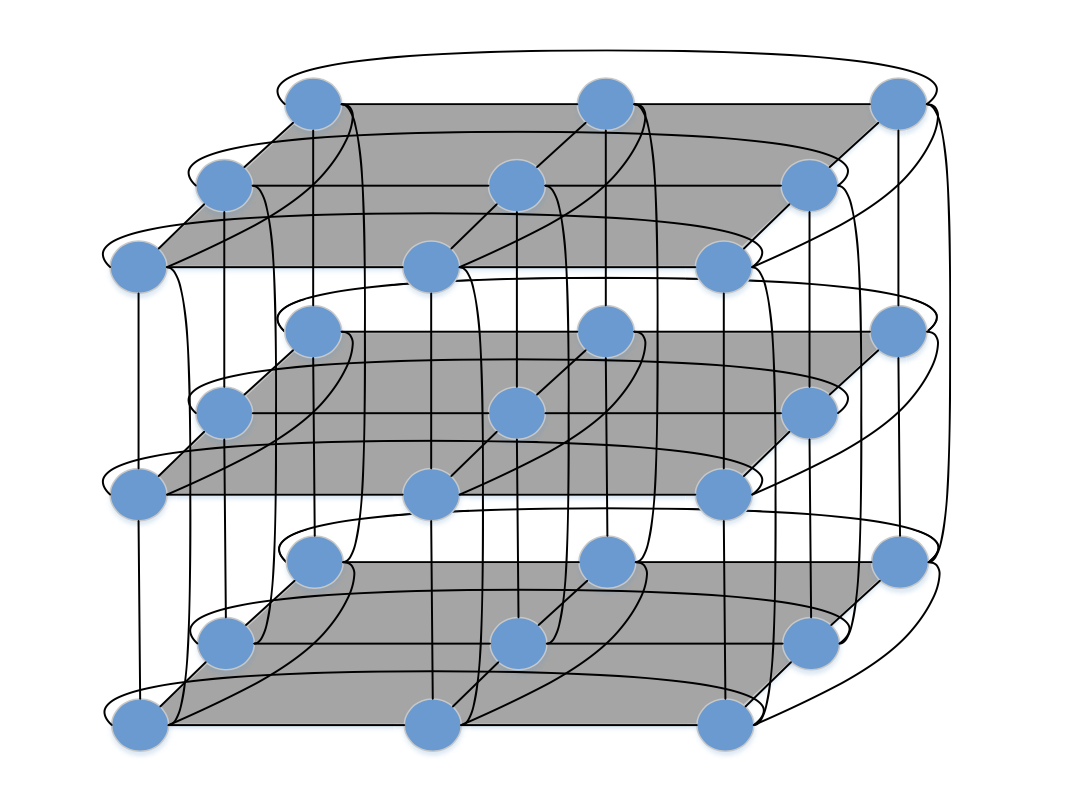
\includegraphics[height=4.5cm]{figure/camcube.png}
    \caption{CamCube架构,蓝点为服务器 \cite{costa2012camcube}}
    \label{fig:camcube}
    \end{figure}
    
    \item \textbf{BCube}:BCube是一种使用服务器与交换机共同实现数据转发的混合型架构。其结构可以递归地定义:\textit{$BCube_0$}由连接在一个n端口交换机的n台服务器组成;\textit{$BCube_1$}由n个\textit{$BCube_0$}组成,它们与n个n端口交换机相连;\textit{$BCube_k$} ($k \geq 1$)由n个\textit{$BCube_{k-1}$}组成,它们与$n^k$个n端口交换机相连。n=4的情形如图\ref{fig:BCube}所示。BCube架构可以以较低开销提供很高的对分带宽 (bisection bandwidth),但其缺点在于它的递归深度受限于服务器的网络接口控制器(NIC)。
    \begin{figure}[h]
    \centering
    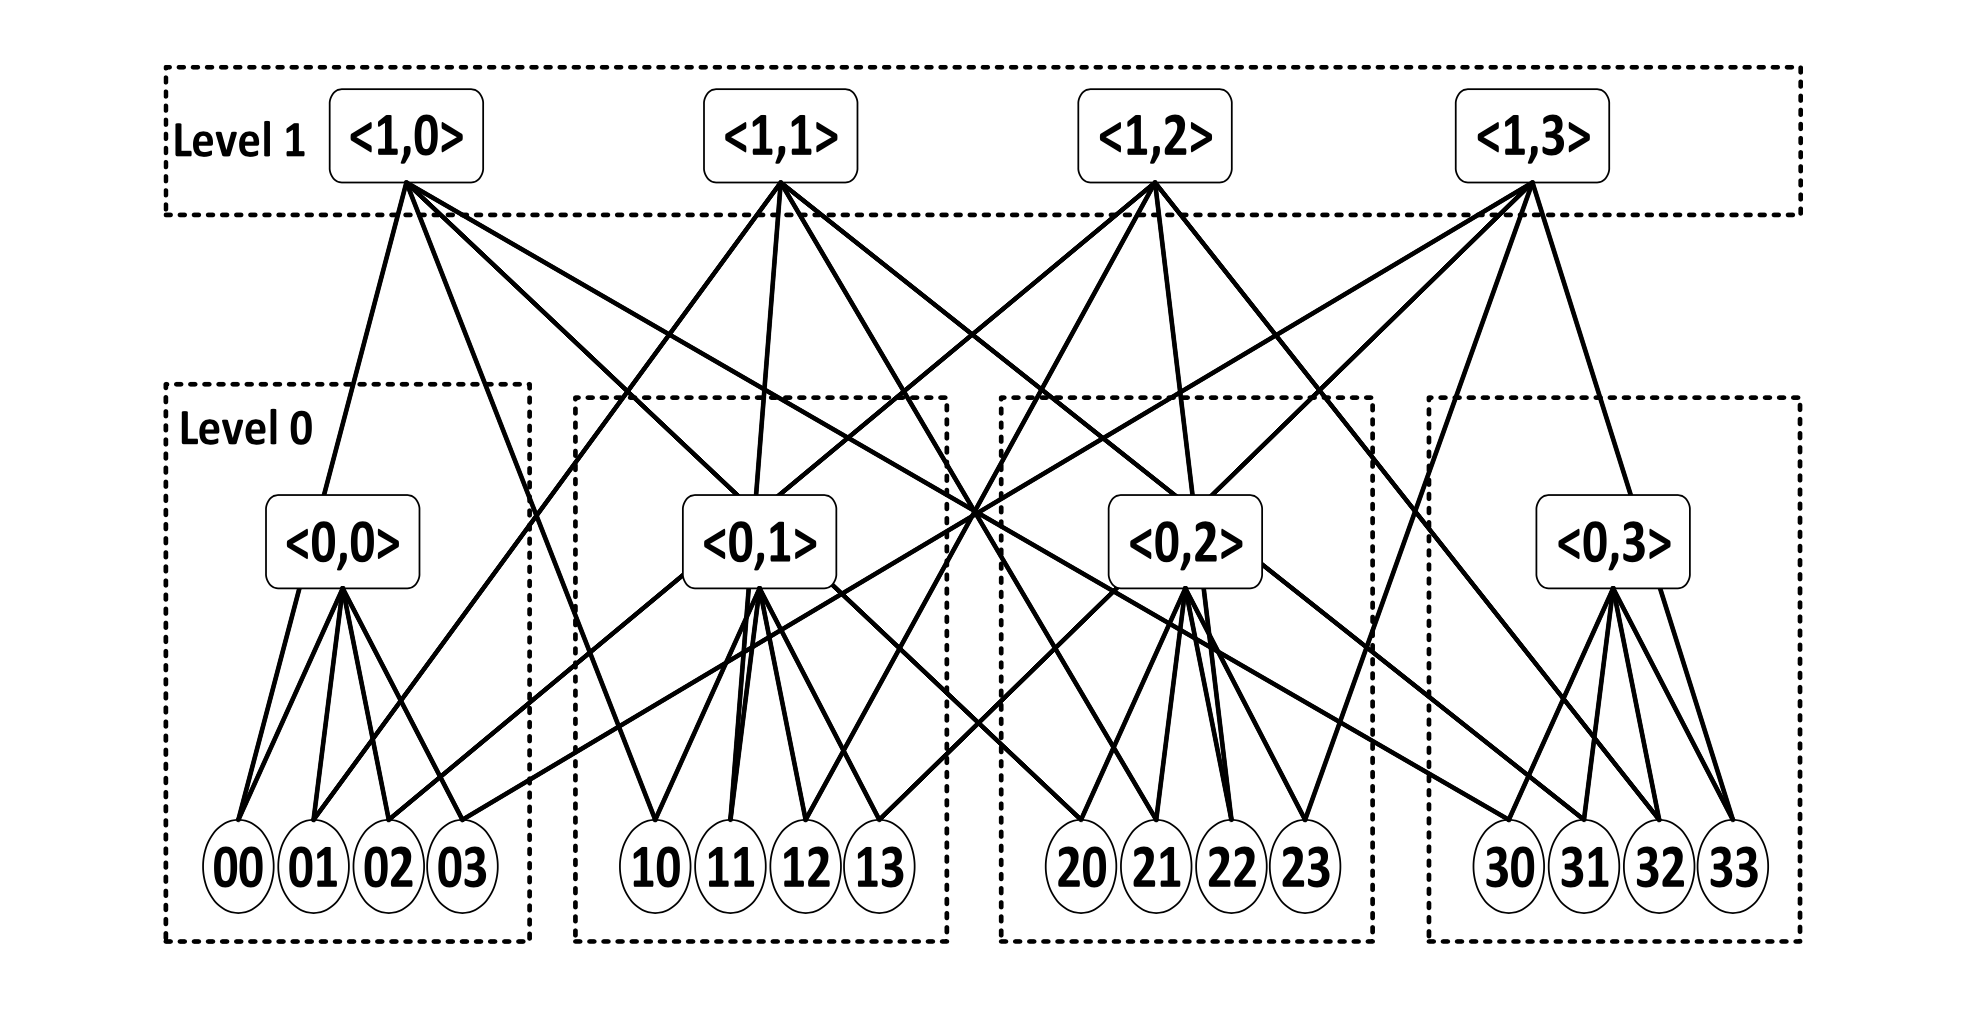
\includegraphics[height=4cm]{figure/BCube.png}
    \caption{BCube架构,图中方框代表交换机,圆圈代表服务器 \cite{guo2009bcube}}
    \label{fig:BCube}
    \end{figure}
    
\end{itemize}

\subsection{流量特征}
数据中心网络中运行着很多不同的应用,从对低延迟有较高要求的网页搜索任务,到类似数据库更新的这种有着高吞吐量要求的任务。通过对于Netflow\cite{netflow2018}和SNMP\cite{benson2010under,benson2010network,greenberg2009vl2}数据的分析可以看到数据中心的流量特征。首先,数据中心的流量目的地与拥有者有关:在云数据中心,近80\%的流量属于其机架的内部转发;学校和私营企业的数据中心,40\%-90\%的流量穿越在不同的机架间。这是由于云数据中心的应用被很好地部署在各机架上以避免机架间的数据传输。第二,数据中心内的大部分数据流都很小(几KB),并且这些数据大部分是分布式系统中的元数据(meta-data)请求。只有少量数据流的大小是100MB到1GB,几个GB的数据流极少。第三,尽管数据中心的大部分数据流都较小,总体数据中大部分还是由大数据流构成,即大数据流的数目少,却占了数据中主要的部分。最后,源头为数据中心机架上的数据本质上是类似于受开关函数控制的流量,开关函数是符合重尾(heavy-tailed)分布的。然而总体的流量分布是随机的、不可预测的。

对于数据中心的拥塞问题,从直觉来说,丢包率与链路的利用率成正相关,但最近的研究表明,二者之间没有关联,是某些流量模式导致了严重的丢包率\cite{zhang2011modeling}。另外,链路的利用率在更高层中增长迅速\cite{benson2010under,benson2010network},例如:核心层中的链路利用率经常达到70\%,然而核心链路的丢包率却是惊人的少\cite{benson2010under}。研究表明,数据包的丢失主要由每一层的微小流量突发造成,并且边缘层中的突发数据比核心层中更多。另外一个特征是,由于拥塞问题,一小部分链路总是比数据中心的其他链路经历更多的丢包,这种情况可以通过部署适当的负载均衡算法得以解决。通常,数据中心会部署备用设备和多余的链路以保证高可靠性,但设备或者链路的损坏在数据中心依旧时有发生,其可靠性与网络的拓扑结构相关。我们希望负载均衡算法能够对网络组成部分的损坏情况做出快速反应。我们注意到有关网络组成部分的损坏的一些特征:1)即便是价格低廉的路由器也非常可靠;2)软件的错误既可以导致设备损坏也可能导致链路的断开;3)链路断开会导致大量的包丢失,并极大影响TCP的性能;4)网络中的冗余链路可以减缓链路断开的影响。然而,当前的流量调度、负载均衡算法难以动态利用数据中心的冗余链路。这是因为当前的算法主要借鉴了静态的较为稳定的网络架构中成熟的均衡算法(如等价多路径算法\footnote{Equal-Cost Multipath Routing,缩写为ECMP}和多协议标签交换\footnote{Multi-Protocol Label Switching,缩写为MPLS})。一个好的均衡算法应当考虑到上述数据中心网络的特征。具体来说,该机制应当以微秒级的速度传输大的数据流,并以更快的速度传输小数据流;应当能动态的对链路的断开进行实时调整,将数据流引向拥塞情况不严重的链路上。

\section{负载均衡问题}

负载均衡是人们长期以来关注的课题。它存在于各个场景下:基于因特网的服务\cite{hong2006dns}(域名系统委派\footnote{Domain Name System (DNS) delegation}中的负载均衡;客户端或服务器端的负载均衡等)、数据中心网络\cite{alizadeh2014CONGA}(服务器之间存在多条路径导致的流量分布不均等)、无线通信系统(处理冗余的通信链路等)。在不同的场景下,鉴于所期望实现的不同目标,研究者们设计了各种负载均衡算法。从研究这些算法思想的过程中,可以汲取一些思路,并学习如何在特定情况下进行仿真实验以验证算法的有效性。

传统蜂窝网络中的负载均衡算法被广泛研究,如小区呼吸技术\cite{niu2010cell}已被应用于第二代和第三代移动通信网络中。由X. Lin和S. Wang提出的Cloud RAN中的高效RRH切换机制在考虑系统能效条件下\cite{lin2010efficient}实现了负载均衡。C. Ran和S. Wang等人从另一个角度提出了Cloud RAN中的最佳负载均衡算法:他们周期性地监控衡量均衡度的公平指数,当其低于特定阈值时,则重新设计每个小区覆盖的区域以实现系统的负载均衡\cite{ran2015optimal}。C. Tsai和M. Moh在Cloud RAN架构下比较了8种均以降低物联网\footnote{Internet of Things,缩写为IoT}设备通信延迟为目标\cite{tsai2017load}的负载均衡算法。由于本文主要考量5G通信系统内数据中心网络中的负载均衡问题,这里对传统无线通信系统中的相关问题不做过多的讨论。

\section{数据中心网络中的负载均衡算法}
我们知道,在5G无线通信系统中,数据中心网络是基站技术不可或缺的关键组成部分,这一小节主要研究数据中心网络中的负载均衡算法。数据中心网络通常为各种应用提供对分带宽 (bisection bandwidth)而采用可横向拓展的模型\cite{zhang2018survey},大量数据在网络中的服务器间通过多条路径传输。基于前面提到的数据中心网络的数据流量特性,本节首先讨论数据中心网络负载均衡的定义、特征、目标,之后比较数据中心网络与广域网\footnote{Wide Area Network,缩写为WAN}中负载均衡的不同,最后引出本文主要场景下的负载均衡算法。
\subsection{定义、目标与主要步骤}
容量受限的网络中的流量调度可以建模成一个被深入研究过的问题:多商品流问题\footnote{Multi-Commodity Flow,缩写为MCF}。数据中心网络的流量调度问题就是找到如下MCF问题的最优解:
\begin{itemize}
    \item $ maximize: \sum\limits_{i}U_i(x_i)$
    \item $\sum\limits_{u:(s,u) \in E}f_{u,v}^{s,d} = \sum\limits_{w:(v,w)}, \forall v,s,d$
    \item $\sum\limits_{u:(s,u) \in E}f_{s,u}^{s,d} = \sum\limits_{i:s \rightarrow d}x_i, \forall s,d $
    \item $\sum\limits_{s,d}f_{u,v}^{s,d} \leq c_{u,v}, \forall (u,v) \in E $
\end{itemize}

其中,目标函数$\sum\limits_{i}U_i(x_i)$代表“商品的效用”,它取决于流的发送速率。$x_i$是流$i$的发送速率。$f_{s,u}^{s,d}$是链路$(u,v)$上的流速率,$(s,d)$代表了流的源地址和目的地址。负载均衡问题本质上是对流进行链路分配,只依靠负载均衡不能保证MCF问题的最优解,这是因为最优的策略与流的发送速率有关。通常情况下,发送速率由端系统的传输控制协议(如TCP)决定。在一个具有固定发送速率的对称网络\footnote{对称网络是指网络中对于所有的源端-目的端对(s,d),s和d之间最短路径上的所有到源端s距离相同的交换机到目的端d都有相同的容量}中,负载均衡算法等价于对最大链路利用率的最小化问题的求解:$\min \max\limits_{(u,v) \in E} \frac{\sum\limits_{s,d}f_{u,v}^{s,d}}{c_{u,v}} $。不过,由于MCF问题是NP-hard问题,难以在微秒级的时间内得到最优解,负载均衡问题需要依靠先验性的算法解决。

%在数据中心网络中,调度的粒度可以分为三种,单流,flowlet,以及固定长度的flowcell。
Jiao Zhang等人\cite{zhang2018survey}提出,数据中心网络负载均衡的主要目标可以分为四类:高性能、可扩展性、鲁棒性、能效。

\begin{itemize}
    \item 高性能:吞吐量和延迟是高性能目标的两个要求。如前文所述,数据中心内的大部分数据来自较大的流,因此算法的表现主要取决于均衡机制对大流的处理上。不同于网络运营商的考虑(他们更关注于吞吐量),数据中心的用户主要关注低延迟的问题。Amazon的调研指出,每100ms的延迟就会导致销量下降1\%。延迟的主要因素是不平衡的流量分配,即在链路中较小的流可能会被较大的流堵住,而致使流完成时间\footnote{Flow Completion Time,简称为FCT}的急剧增加。
    \item 可扩展性:随着数据中心运行起越来越多的应用,其规模近年来不断扩大。由于大多数负载均衡机制要求存储链路利用信息,如CONGA使用叶节点交换机维持一个每条路径的拥塞情况表,当数据中心规模增加时,可能存在用尽边缘交换机内存的风险。另外如果均衡机制是针对某种架构设计的,如CONGA是为2层拓扑结构设计的,那么将其应用到三层结构中,拥塞信息可能就无法准确地收集。
    \item 鲁棒性:即便数据中心使用的设备都较为可靠,链路的断开与交换机的损坏依旧时有发生;经常性的软件或硬件更新会导致网络拓扑结构的改变,这会导致端系统间的链路发生改变。上述问题均是负载均衡算法需要面临并解决的问题。目前主要有两种解决方案:一种是使用一个中心控制器周期性地监控网络状态,当错误发生或网络结构改变时,中心控制器改变负载均衡算法以做出合适的调整;另一种在交换机处分布式地监视端口信息,当错误发生时或结构变化时将端口设置成不可用状态。
    \item 能效:数据中心的能效问题日益受到关注,由于数据中心提供大量的对分带宽和多条备用链路,这些冗余会造成大量的能量损耗。尽管相关研究指出\cite{koomey2011growth}最近几年数据中心的能耗增长逐渐放缓,维持一个数据中心的运行的成本也是极其惊人的。主要有两种途径减少能量损耗:根据工作负载的特性,关闭没在使用的设备(
    如动态能量管理机制DPM),以及降低设备的性能(如动态电压频率调整机制DVFS)。
\end{itemize}

一般而言,负载均衡机制可以分为两个主要步骤:收集拥塞信息和选路。

\textbf{(1)收集拥塞信息}

负载均衡机制需要根据拥塞信息(如链路利用率、显示拥塞指示\footnote{Explicit Congestion Notification,缩写为ECN}等)来确定数据流的路径,也就是说负载均衡的一个关键步骤是要选择一种或多种代表拥塞信息的衡量标准,并将它传送至为数据流做选路决定的实体。收集拥塞信息的方法有以下三类:
\begin{itemize}
    \item 基于TCP的采集:TCP将数据包的丢失视为网络拥塞的信号,并且当检测到拥塞情况时会减小拥塞窗口。基于TCP的采集方法(如MPTCP\cite{raiciu2011MPTCP},CLOVE\cite{katta2016CLOVE}等)利用与TCP或TCP变种相似的信号检测拥塞情况,ECN就是负载均衡中常用的一种信号。
    \item 发送速率:数据流的发送速率是可以由交换机和端系统直接检测到的数据。基于各个数据流已发送的数据量,可以在时间上控制不同数据流的发送,以此实现所有数据流的平均发送速率。由此,基于发送速率的方法(如Hedera\cite{fares2010hedera},CONGA\cite{alizadeh2014CONGA},LocalFlow\cite{sen2013LocalFlow},Fastpass\cite{perry2014Fastpass})就根据已发送的数据量判断拥塞情况,通常在软件定义网络\footnote{Software Defined Network,缩写为SDN}中使用较多。这是因为其中的OpenFlow交换机自动地记录已发送的数据量,且控制单元可以随时访问这个量。
    \item 交换机的队列长度:交换机缓存的利用率是流过该交换机的数据流的直接反映。基于交换机队列长度的方法(如Expeditus\cite{wang2014Expeditus},DRILL\cite{ghorbani2015drill})利用路径上交换机的队列长度代表链路的利用率、检测拥塞情况。这种方式对于内网的情形较为方便。
\end{itemize}


\textbf{(2)选路}

在获取数据中心网络的拥塞信息后,负载均衡机制需要对到达的数据流分配不同的路径以实现各路负载的平衡。在不同的场景下,负载均衡机制的目标与算法略有不同,以下列举了四种选路的方式:
\begin{itemize}
    \item 拥塞最少:最理想的选路方式是把每个数据流分配到最不拥塞的链路上。因此这种方式可以通过收集每条路径的拥塞信息并将数据流传送至拥塞最少的路径上。这种方式(如CONGA\cite{alizadeh2014CONGA},Expeditus\cite{wang2014Expeditus})的性能与链路利用率的响应时间与准确性密切相关。
    \item 较少的拥塞:由于很难实时采集链路利用率的准确值,另一种方式是将数据流从拥塞情况严重的路径转移到拥塞情况较轻的路径上去,同时减少了记录所有路径信息的开销(如MPTCP\cite{raiciu2011MPTCP},DRILL\cite{ghorbani2015drill},Hedera\cite{fares2010hedera})。
    \item 轮询调度:原始的轮询调度是将数据流一个一个地分配至所有可行的路径。由于它对数据流和链路信息不可知,在重负载情况下很容易产生流的碰撞。因此可以根据数据流的长度和链路利用率采用加权轮询的方式均衡分配,此种方法(如CLOVE\cite{katta2016CLOVE},Presto\cite{he2014Presto})的性能受到链路权重的影响。
    \item 集中式分配:以上提到的三种方法,对于每个数据流的选路过程彼此间相互独立,这可能会导致局部最优的情况。因此集中式分配的方式对数据流进行整合式的分配以达到全局最优(如Fastpass\cite{perry2014Fastpass},LocalFlow\cite{sen2013LocalFlow})。
\end{itemize}
\subsection{数据中心与WAN中负载均衡的比较}

在很多方面,数据中心与WAN中的负载均衡问题是相近的,比如问题的定义,比如二者均是对多条链路分配网络流量等,然而二者之间有很多的不同点:
\begin{itemize}
    \item WAN中的网络拓扑结构通常是不规则的,而数据中心的网络结构通常是对称的,即在每对端系统间的链路是equal-cost的,这提供了高对分带宽并减少了计算链路的复杂性。
    \item WAN可能包含不同的链路容量和硬件种类,因此流量调度机制就要求将不同结点的限制考虑进去。对比之下,在数据中心的一层中,交换机常常是一种类型的,链路容量也完全相同,这极大地简化了问题。
    \item WAN中服务与调度的变化通常要花数小时或者数天,而在具有高速链路的数据中心,较小的流只需要数十或者数百毫秒进行传输,数据突发所导致的拥塞可能在毫秒级的时间内就消失了,这就要求流量调度算法足够及时地处理拥塞情况。
    \item WAN通常没有中心控制器,全局的网络信息难以被收集、链路断开难以被解决,而数据中心采用的一些可编程架构,如SDN,都提供了中心控制器,以对网络的全局信息进行收集与处理,因此可以提供中心化的实时流量调度。
\end{itemize}

通过比较WAN和数据中心网络,可以更清晰地看到数据中心网络负载均衡的特殊环境。具体来说,数据中心的网络结构更有规则,数据流量变化更快,中心化的控制比较常见,这为负载均衡算法留出了更多的设计空间。

\subsection{近年来提出的负载均衡算法}

本小节从分布式和集中式的分类角度介绍近年来提出的负载均衡算法。这两类机制的主要区别在于是否有一个中心控制器采集拥塞信息并实时为数据流选路。对于集中式机制,中心控制器可以容易地获得全局的链路利用信息,但通常都需要额外的开销向控制器传送信息,此外,集中式算法的时间粒度较分布式而言比较粗糙,大部分集中式的控制器都得不到最及时的信息以处理数据中心网络中的数据突发。由于分布式系统中的选路决策发生在端系统或交换机处,这样就可以足够及时地应对数据突发。但通常分布式的算法是为对称网络设计的,当拓扑结构有所改变时(如链路的断开、交换机的崩溃)就很难应对。

\textbf{(1)集中式负载均衡}
\begin{itemize}
    \item Hedera\cite{fares2010hedera}:Hedera是一个主要针对大数据流处理的集中式算法。由于ECMP不能很好地处理大数据流,甚至会造成流的碰撞,Hedera提出了一种估计大数据流并中心化地对其分配路径,以最小的开销使网络利用率最大化。具体而言,Hedera的第一步是在边缘交换机处检测大数据流,第二步是根据分配算法为这些大数据流选路,最后,控制器在相关的交换机上部署路径信息。在检测数据流的阶段,中心控制器在边缘交换机处周期性地监测流速率,当一个数据流的速率大于链路容量的10\%,则认为它是一个大数据流。大数据流的选路有两种方法:全局优先匹配和模拟退火算法。全局优先匹配为大数据流选择一条能够容纳该数据流的链路,这种方式适合工作在负载较轻的网络中,当网络负载增加、链路饱和时则不能保证所有的数据流都满足预设条件。模拟退火算法将目的地址相同的大数据流集合起来,并为它们分配一个核心交换机,这可以极大地减小控制器的搜索空间。这种算法每次处理一批数据流,采用迭代机制寻找最优的分配方式。在选路之后,控制器将相应的转发规则通过OpenFlow协议部署在相关的交换机上。当链路发生断开情况,Hedera通过使用可扩展、可容错的2层路由转发协议PortLand\cite{mysore2009Portland}解决这一问题。仿真结果显示在平均对分带宽上Hedera比ECMP表现更好,且其头部开销是可接受的,流速率估计过程的复杂度与端系统和大数据流的数量呈正相关。全局优先匹配与模拟退火算法的运行时间为数十至数百毫秒,这符合数据中心对于处理速度的要求。然而,并不是所有的大数据流都会达到速率限制,Hedera中的大数据流检测方法可能是不准确的。另外,除非当一个大数据流达到速率限制,它才会被分配一个合适的路径,这会导致一些数据包的安排不合理。至于控制过程,尽管数据采集与大数据流调度可以很快地完成,仿真过程中整个操作流程花了5秒,对于数据中心网络,将其减小到200毫秒是比较合理的,但这会增加额外的开销,实际中部署起来也较难实现。
\begin{figure}[ht]
    \centering
    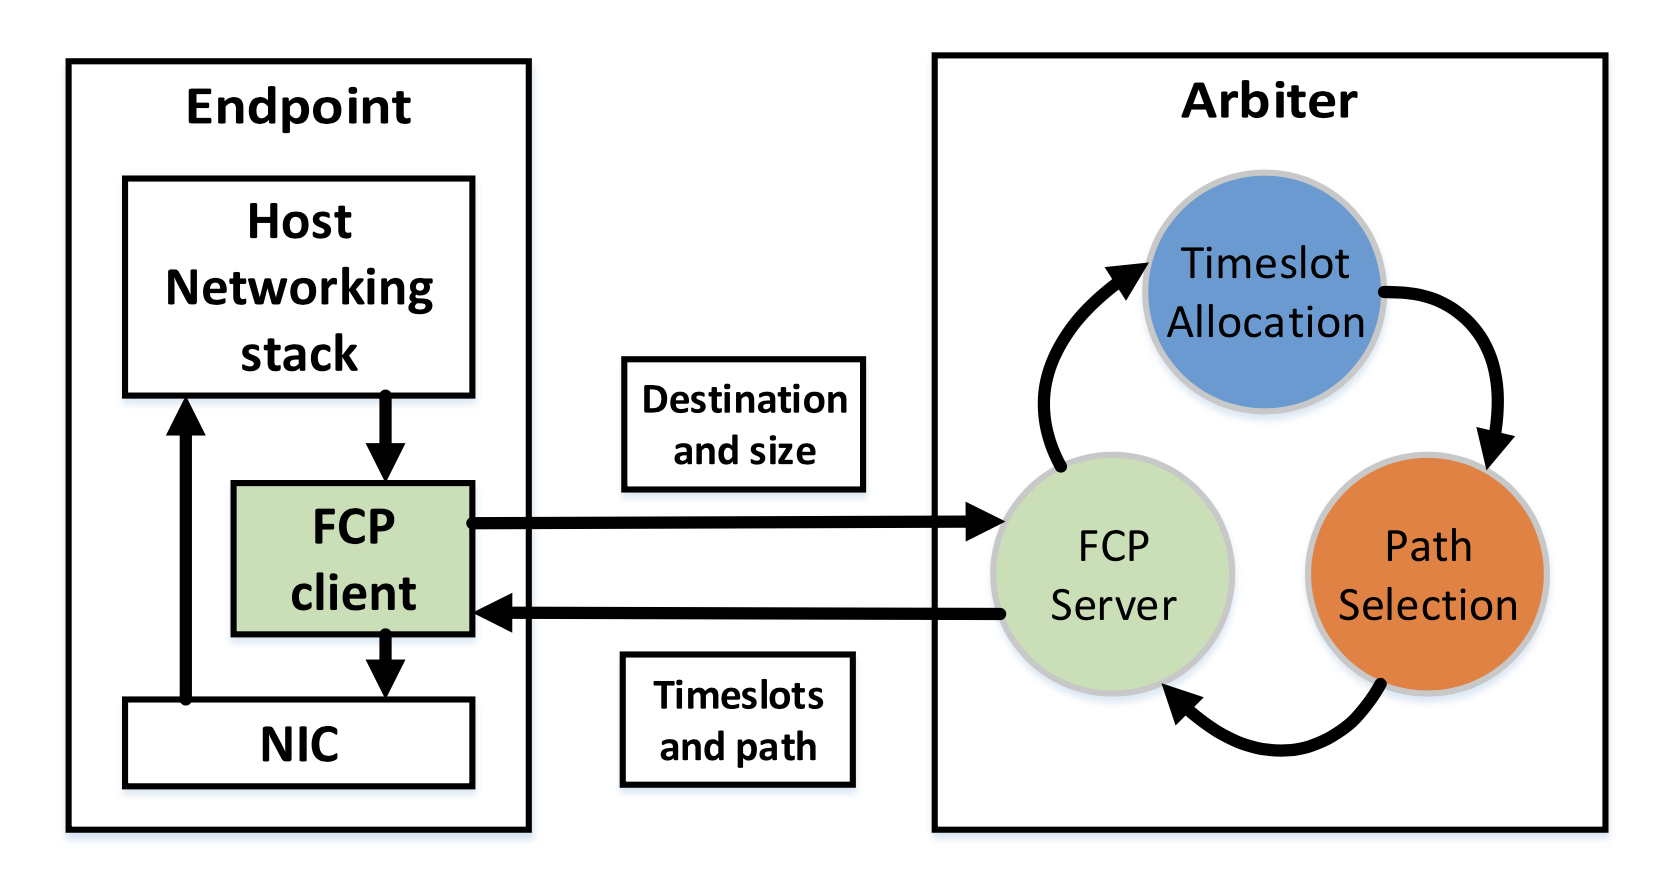
\includegraphics[height=5cm]{figure/Fastpass.png}
    \caption{Fastpass结构图}
    \label{fig:Fastpass}
\end{figure}
    \item Fastpass\cite{perry2014Fastpass}:Fastpass是一个混合型的负载均衡机制,它将传输控制和流量的调度相结合以达到数据中心网络的"零队列"(zero-queuing)。Fastpass控制每个数据包的发送时间和传输路径,其主要的组成部分是时间片分配和选路机制\ref{fig:Fastpass}。其中,Fastpass控制协议(英文简称FCP)负责传输数据交互的需求和时间片的分配决定。时间片分配这一部分控制着每个数据包发送的时间,以实现最小化FCT的目标,它是流水线的方式实现的:在一个时间片内以尽力服务的模式实现一部分数据交互的需求,另一部分的需求要等到下一个时间片处理。之后,选路算法为已分配时间片的数据包指定零队列的发送路径,该算法采用图论中的边染色算法(以一个二分图作为输入,为图的每条边染色,使得同一结点上的两条边颜色不相同)。针对网络结构的变化,Fastpass采用replication策略以应对链路断开或者控制器的出错。具体而言,端系统向一个错误隔离机制报告数据包的丢失,该机制继续向控制器上报,此时控制器就会避免向这个出错的部分分配流量。当控制器出现问题时,备用的控制器就会取代之前的控制器继续流量调度。与\cite{perry2014Fastpass}中提到的一个采用TCP协议的基准算法相比较,Fastpass可以明显减少队列长度和FCT,并达到较高的吞吐量。Fastpass的主要弱点是部署较难,可扩展性不好。由于中心控制器需要为每个数据包决定时间片与发送路径,Fastpass的性能主要由控制器的处理速度决定。单个控制器可以处理数百或数千个端系统的均衡问题,但对于拥有更多端系统的大型数据中心网络,单个控制器的计算资源可能会成为瓶颈,因此可能需要多个控制单元的合作。多控制器的架构以及如何保持数据的一致性亦是目前研究的热点\cite{dixit2013towards,berde2014onos}。
\end{itemize}

\textbf{(2)分布式负载均衡}
\label{sec:loadBalance}
我们共列举七种主流的分布式负载均衡算法,其中前四种是已知拥塞信息的均衡机制,它们均通过采集拥塞信息做出基于全局的流量调度;后三种是拥塞信息未知条件下的均衡机制。
\begin{itemize}
    \item MPTCP\cite{raiciu2011MPTCP}:多路径TCP(英文简称MPTCP)是一种根据拥塞信息做出相应均衡决策的机制。它利用端系统之间的多条路径并设置多个子链接来充分利用带宽、提高吞吐量。MPTCP使用SYN来确定使用该机制,在成功建立TCP连接后,客户端从SYN消息得知服务器具有的额外IP地址或TCP端口,这样就可以使用不同IP地址或端口建立额外的连接。在传输过程中,每个MPTCP子流有其独特的序列号并维持一个拥塞窗口。此外,MPTCP修改了TCP中的一些特征,以使多个子流同时工作。\cite{raiciu2011MPTCP}通过仿真实验得到,与TCP相比,MPTCP极大提升了数据中心的吞吐量。但MPTCP有两个主要问题:1)数据中心网络的大部分数据流都比较小,将它们分解成子流以使用额外的TCP连接实际上增加了FCT。另外在某些情境下,使用多条链路(与使用单条路径相比)只能带来较少或有限的增益。2)MPTCP在为子流选路上依赖于ECMP和其他路由机制,如果某些子流被分配至拥塞的路径上,其效果就会下降。FMTCP\cite{cui2015fmtcp}和A-MPTCP\cite{Coudron2013AMPTCP}是两个针对MPTCP性能提升的机制。
\begin{figure}[ht]
\centering
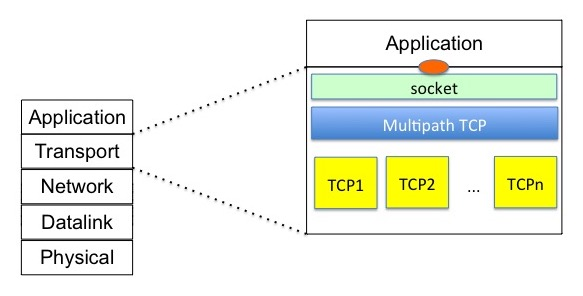
\includegraphics[height=5cm]{figure/Multipath_TCP_architecture.jpg}
\caption{MPTCP在协议栈中的位置}
\label{fig:MPTCP}
\end{figure}
    \item CONGA\cite{alizadeh2014CONGA}:CONGA是为两层叶脊(leaf-spine)拓扑网络设计的最佳负载均衡机制。其设计者指出:集中式机制对于拥塞情况的反应太慢、单纯的局部机制又很难收集到全局拥塞信息,因此他们设计了一种能够在叶结点交换机上收集全局拥塞信息的分布式算法,他们利用VxLAN\cite{maha2014VxLAN}虚拟化技术承载链路利用率信息,使用VxLAN头域中额外的四个标记,将拥塞信息通过数据包从目的叶结点交换机传送至源叶结点交换机。为了记录链路的拥塞信息,每个叶结点交换机维护目的地址拥塞表。每当反馈信息到达交换机就更新一次该表。此外,CONGA将数据流分成flowlet以实现较少数据包重排的细粒度负载均衡目标。一个flowlet是由叶结点交换机监测判断的,即当两个连续数据包之间的时间空隙超过了路径导致的最大延迟时,则判断前后数据包为两个flowlet,否则为同一个flowlet。flowlet由叶结点交换机维护的拥塞信息表指定一条拥塞最少的路径进行传输。CONGA与ECMP和MPTCP进行了性能比较,结果显示CONGA实现了比ECMP和MPTCP更少的FCT(在企业负载和数据挖掘负载任务上有或无链路断开故障),且在incast场景下CONGA的吞吐量是MPTCP的2-8倍。然而CONGA也有不足之处:1)首先它要求对叶结点交换机和VxLAN的头部进行修改,这对于目前的数据中心实现起来有一定困难;2)CONGA还需要花几个往返时延\footnote{Round-Trip Time,简称为RTT}(数十至数百微秒)等待拥塞信息的反馈,对于数据中心而言,可能这段时间内拥塞已经消失了;3)当多个流同时到达交换机处,根据拥塞信息表交换机可能为几个流选择同一条路径,从而造成拥塞。
\begin{figure*}[htb!]
\centering
\begin{subfigure}{0.45\textwidth}
     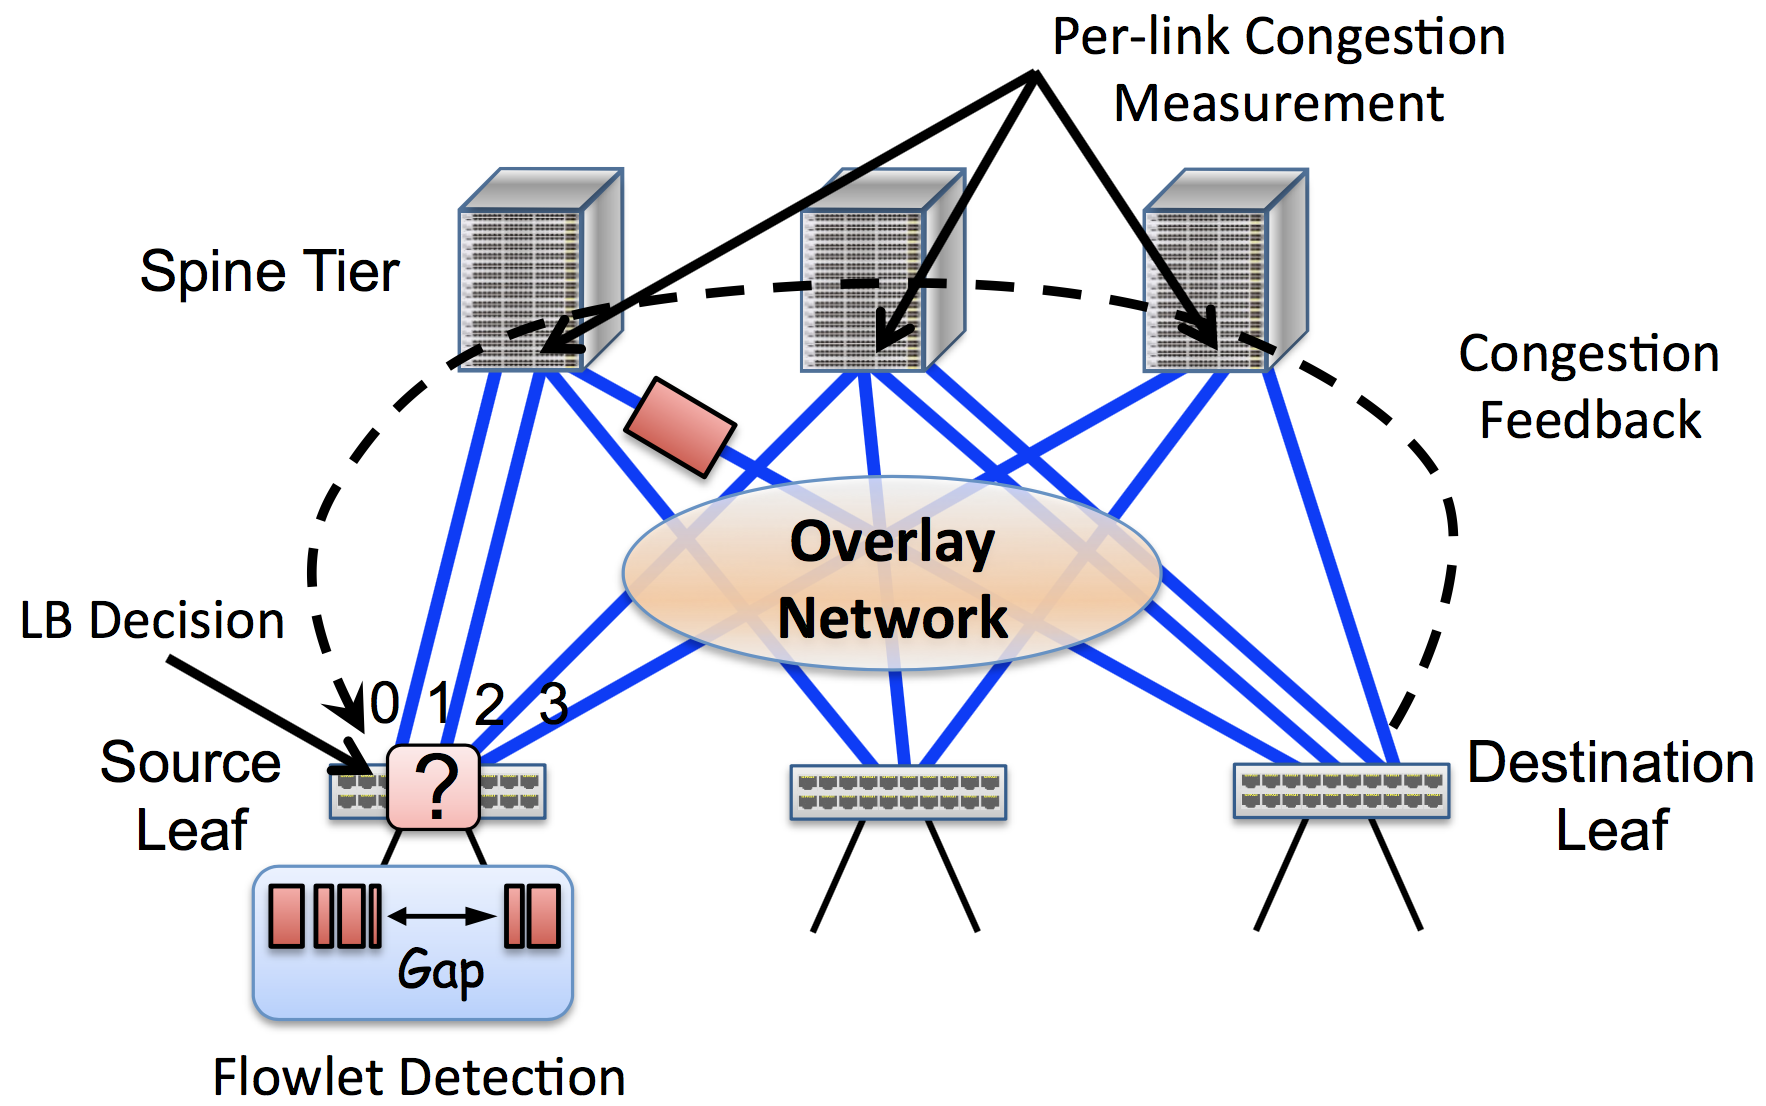
\includegraphics[width=\textwidth]{figure/CONGA_system_archi.png}
    \caption{CONGA的网络拓扑}
\end{subfigure}\hspace{2em}
\begin{subfigure}{0.45\textwidth}
%\centering
    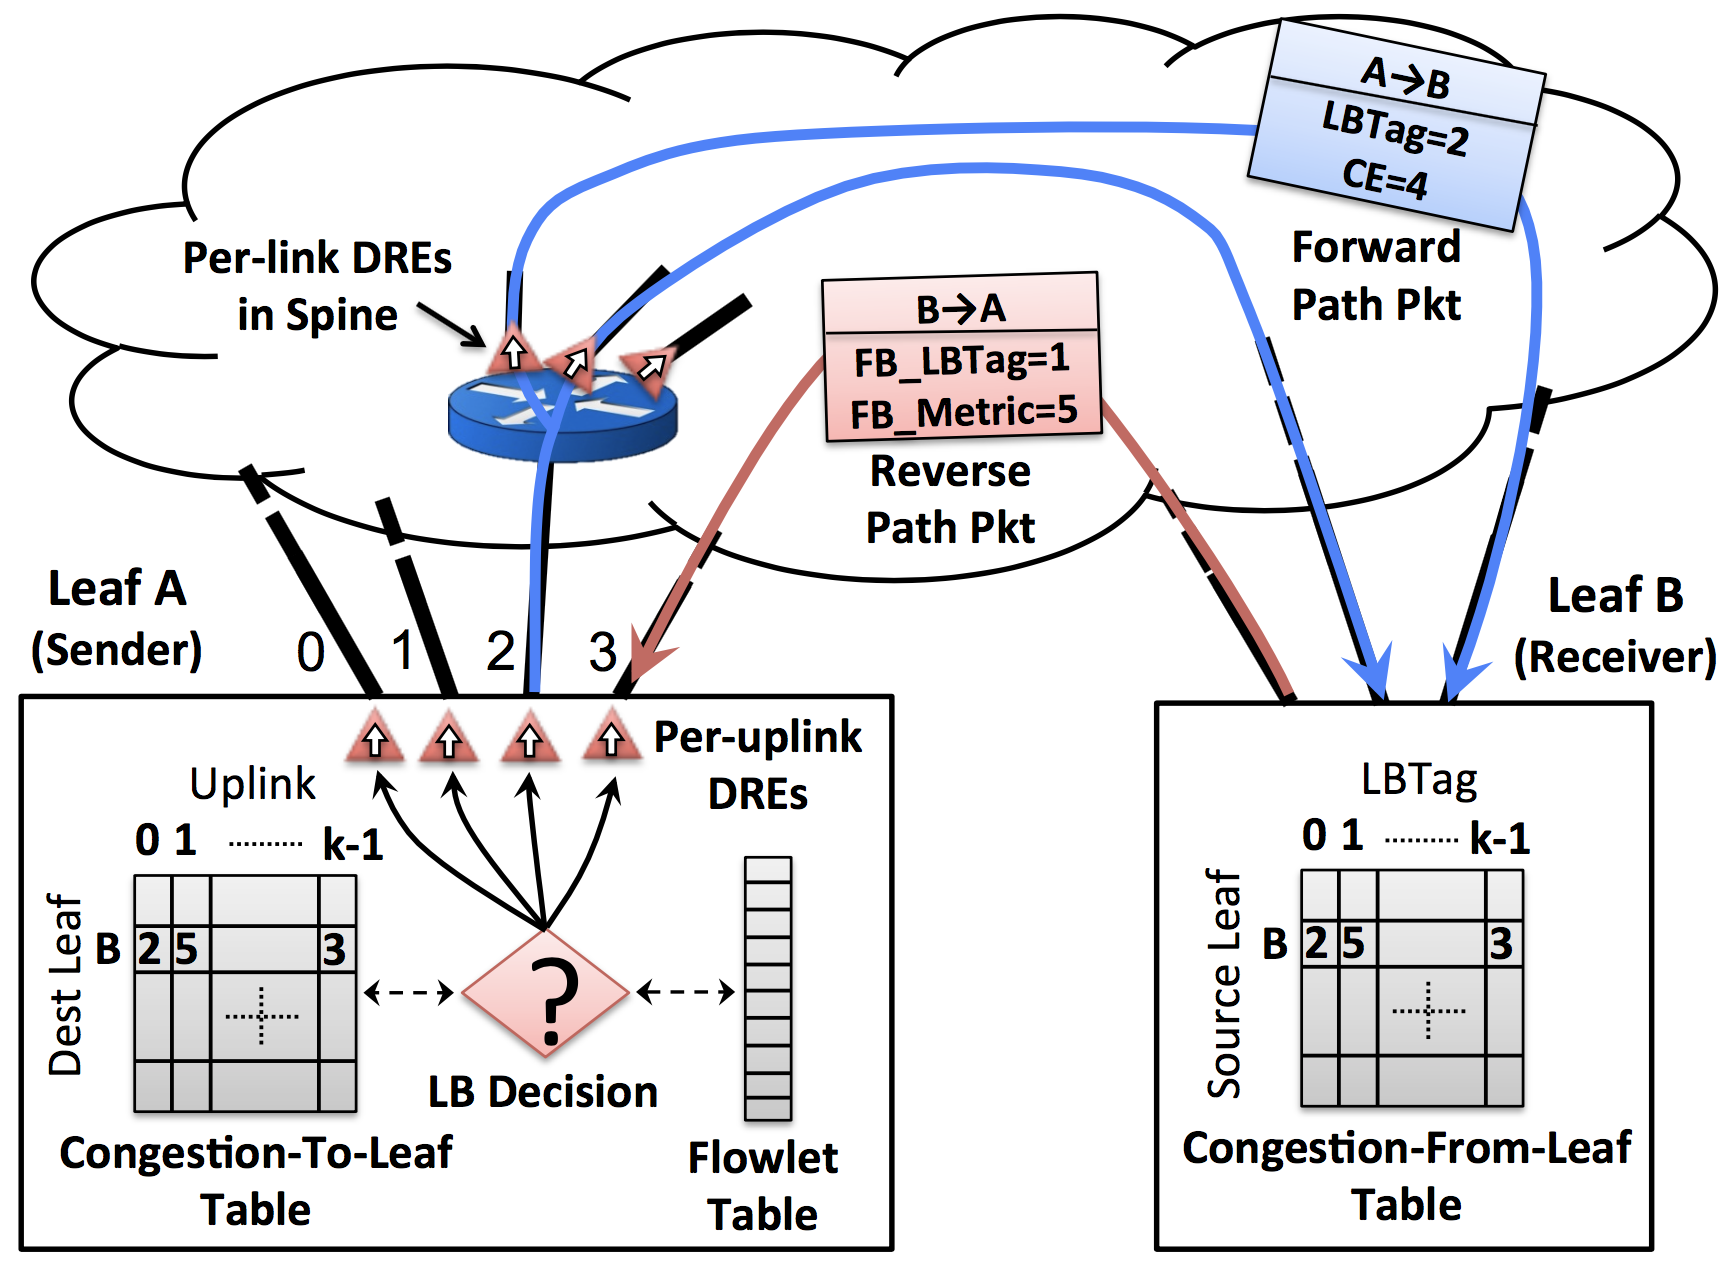
\includegraphics[width=\textwidth]{figure/CONGA_flowlet.png}
    \caption{拥塞信息表}
    
\end{subfigure}%\hspace{0.277em}
\caption{CONGA的主要结构}
\end{figure*}
    \item CLOVE\cite{katta2016CLOVE}:一般而言,集中式的均衡机制对于延迟敏感的短流反应较慢,而分布式的负载均衡常常要修改交换机或端系统的栈。因此,CLOVE选择在交换机的软件上进行修改,以避免对硬件和端系统做改动。CLOVE在物理层上使用标准的ECMP,通过在交换机软件中修改数据包的头部以指导交换机如何传送数据。CLOVE包含三个主要部分,1)路径发现:CLOVE中的交换机软件通过改变源端口地址的方式同时发射许多探头,之后源监视器就可以选择源地址;2)flowlet:CLOVE采用flowlet以避免数据包的重排并在交换机处检测flowlet;3)已知拥塞的路由:CLOVE使用加权轮询机制对flowlet进行均衡。有两种方式得到路径权重:第一种是采用ECN检测拥塞、计算权重的CLOVE-ECN;第二种是使用带内网络遥测技术\footnote{In-band Network Telemetry,简称为INT}精确收集链路利用率的CLOVE-INT。仿真结果显示CLOVE-ECN能够在中等或较重负载下显著提升FCT的平均表现(对比ECMP);CLOVE-INT基本与CONGA的表现相似(不论在对称或在非对称的网络中)。但由于并非所有数据中心网络都使用虚拟化技术,在未采用虚拟化技术的场景下采用CLOVE需要进一步的探究。
    \item Expeditus\cite{wang2014Expeditus}:在例如fat-tree\cite{alfares2008fattree}和VL2\cite{greenberg2009vl2}等基于Clos的架构中,在叶结点交换机处维持拥塞信息通常需要大量的内存,因此,实际上很难实时采集全局拥塞信息。为了解决这个问题,Expeditus针对fat-tree架构提出了两种设计:一跳(one-hop)拥塞信息采集和两阶段选路(two-stage path selection)过程。1)拥塞信息采集:每个交换机既要监视上行(从自身向上游交换机)的链路利用率也要监视下行(从上游交换机向自身)的链路利用率。下行信息通过数据包的头部由出站端口(egress ports)轮询缓存占用率得到。具体而言,当一个数据包从一个核心交换机发出,其包的头部记录了出站端口的速率与核心交换机的IP地址。之后,下游的聚合交换机接收该数据包,获取核心交换机的IP地址,对相应链路利用率进行更新。之后它将核心交换机的IP地址替换为自己的IP地址,轮询出站端口的占用率,更新收包的信息并将它继续向下转发,最后,边缘交换机采用与聚合交换机类似的处理方式将数据包转发给端系统。由下行拥塞信息表记录的占用率若在一段时间内没有更新就会被置为0。2)选路:两阶段选路过程为数据流选择源端到目的端的转发路径和目的端到源端的反向路径。初始状态下,由于交换机处没有拥塞信息,SYN和ACK-SYN包使用ECMP进行路由转发。在第一阶段,SYN包会携带反向路径的拥塞信息至目的端的边缘交换机,因此在接收到SYN包后,边缘交换机就可以选择到达聚合交换机的最不拥塞的反向路径。在第二阶段,SYN-ACk包会携带前向转发路径的拥塞信息到源端的边缘交换机。之后,当SYN-ACK包到达源端聚合交换机时,交换机会决定到达核心交换机的最不拥塞的转发路径。由于目的端的聚合交换机已在第一阶段确定下来,由于fat-tree的结构源端的聚合交换机也随之确定,源端的边缘交换机不需要选择转发路径的源端聚合交换机。Expeditus在叶脊和fat-tree两种架构下与ECMP和CONGA做了性能比较。仿真结果显示在不同场景下,Eepeditus的FCT和末端延迟比ECMP和CONGA降低了25\%到30\%,但是Expeditus对数据中心的网络拓扑有着较严格的要求。
\begin{figure}[ht]
\centering
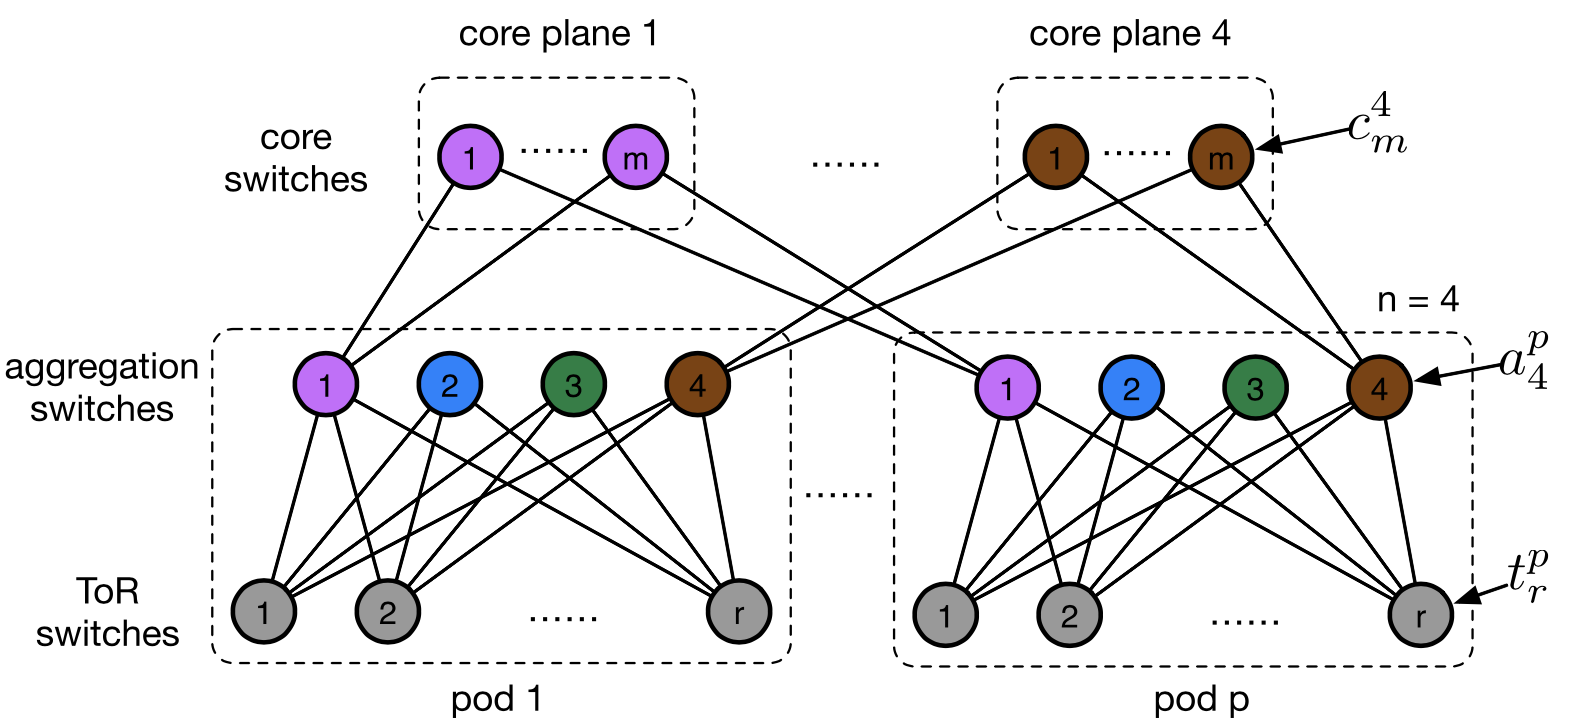
\includegraphics[height=5cm]{figure/Expeditus_archi.png}
\caption{Expeditus的网络结构}
\label{fig:Expeditus}
\end{figure}
    \item Presto\cite{he2014Presto}:Presto同样采用ECMP机制实现非对称拓扑结构中端系统之间数据流的最优均衡。Presto的设计者发现,在对称网络中,如果所有的数据流都是很小的流,ECMP的表现是接近最优的,当数据流的大小分布的标准差变小时,ECMP造成的不均衡情况就会有所减轻。因此Presto将数据流分成等大的小数据流flowcell,并将它们均等地在网络中用ECMP分发。Presto采用TCP数据包分片的最大值\footnote{TCP Segment Offload,简称为TSO}64KB作为flowcell的默认大小,实现了网络中细粒度的负载均衡。Presto的接收端采用通用接收报文\footnote{Generic Receive Offload,简称为GRO}将乱序的包合并为段并将它们组装起来。与ECMP和MPTCP相比,Presto达到了更大的吞吐量和更少的FCT。它可以显著地减少链路断开造成的影响,并在采用加权调度算法时可以达到合理的吞吐量。但是Presto在处理非对称网络时不是最优的解决方案,即便加权算法可以将一些负载从拥塞的路径上调度至其他路径。
    \item LocalFlow\cite{sen2013LocalFlow}:LocalFlow是一个实现在OpenFlow交换机上的本地算法,它提出对每个数据流调度的算法是次最优的,这是因为大数据流不能很好地利用数据中心网络多路径这一特征。通过对每个数据流空间上进行分离并指定合适的路径,LocalFlow在对称网络中表现得很好,已经在大型数据中心得以应用。LocalFlow调度过程是有四个主要步骤的循环体:1)对每个数据流测量速率(使用字节计数器);2)同一目的地址的数据流被聚合成一个大数据流,之后大数据流被分成L个bin,其中L是输出端口的个数,参数$\delta$被用来调整每个bin的大小以减少分流的数量;3)通过对bin大小的排序指定每个bin的输出端口(根据端口带宽),即较大的bin被分至带宽剩余较多的端口;4)控制器更新OpenFlow交换机转发路由表中的规则并重置字节计数器(为下一次循环做准备)。LocalFlow增加了TCP中端系统dup-ACK的阈值来抵消数据包重排的负面影响。LocalFlow被证明是一个在对称网络下可以使MCF优化达到最优情况的均衡机制(如在fat-tree和VL2拓扑中的1024个端系统网络下接近最优)。在由链路断开导致的网络失败情况,LocalFlow也表现较好,与MPTCP8个子流的算法表现相近。实际运用中,LocalFlow的转发路由表只需要很少的空间,这是由于网络中只有较少的数据流需要分解。LocalFlow的主要问题在于它只是比较适合于对称网络中,例如,当高负载或链路断开导致的拥塞已发生时,LocalFlow不能很快地处理,且其调度的间隔较长,应该被缩短至毫秒级的时间以适应现有的数据网络。
\begin{figure}[ht]
\centering
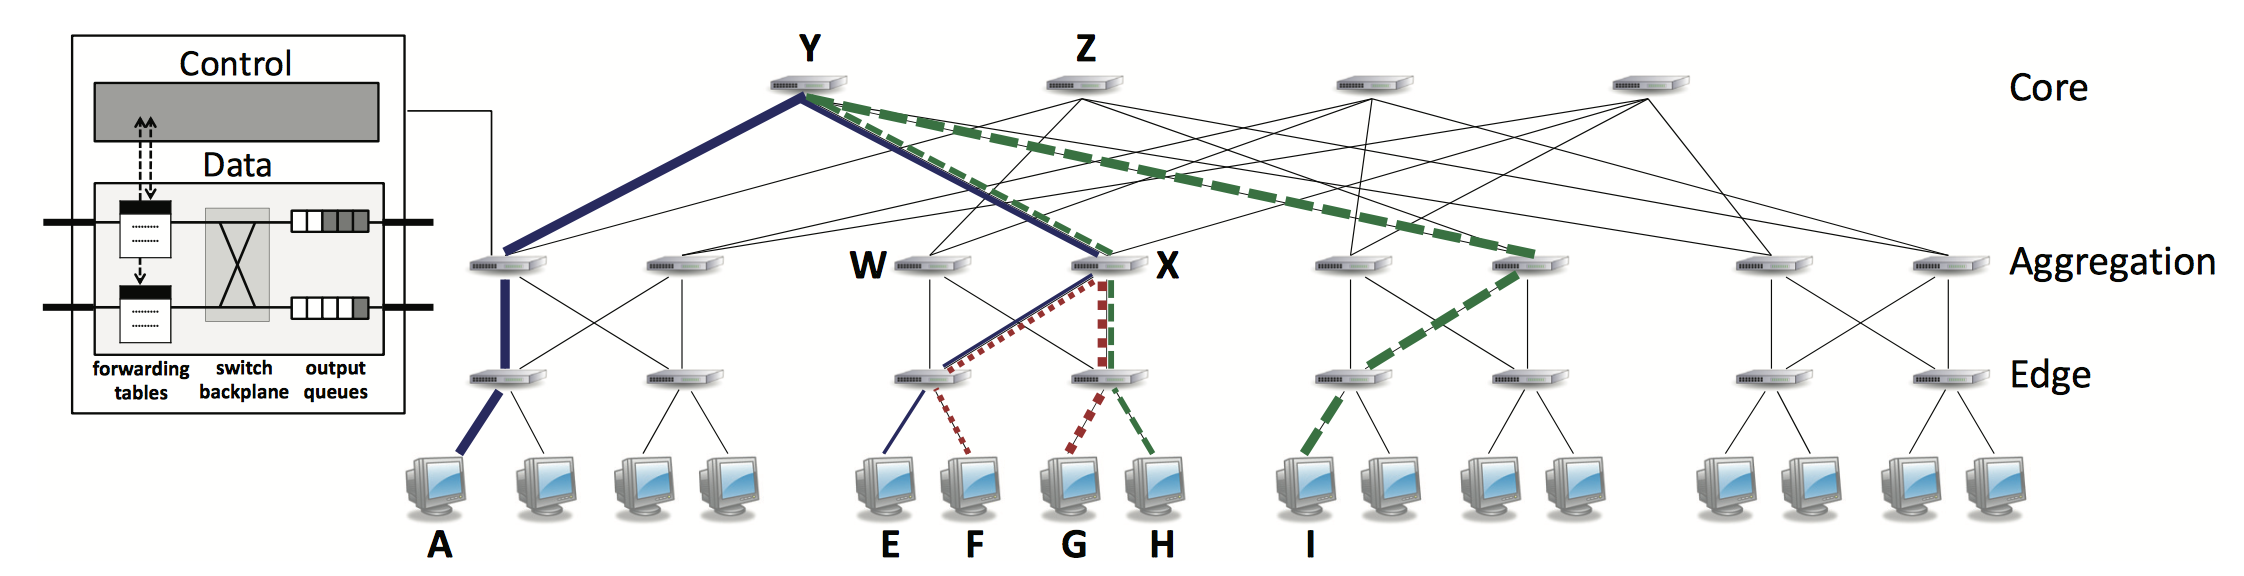
\includegraphics[width=15cm]{figure/LocalFlow_archi.png}
\caption{LocalFlow中的仿真网络拓扑:采用4-端口交换机的fat-tree架构}
\label{fig:LocalFlow}
\end{figure}
    \item DRILL\cite{ghorbani2015drill}:DRILL是一种只运用交换机本地信息的分布式均衡机制,它指出采集全局信息通常会导致较长的控制循环或额外的开销,这难以满足数据中心网络的实时性要求。另外,即便有了全局信息,由于交换机是分布式的、互相不协同工作的,它们可能同时选择了相同的拥塞情况最轻的路径,从而导致这些路径的拥塞。受到超市排队模型中“两种选择的力量”的启发\cite{mitzen2001power},DRILL利用交换机本地信息实现了一种数据包随机分配的机制:当数据包到达DRILL中的每个交换机处,交换机随机选取两个可用端口,将它们的队列长度与一个有记录的端口比较,之后数据包从三个端口中队列最少的端口发送(有记录的端口是指传输上一个数据包的端口)。DRILL中没有额外的开销因而不需要更改硬件与协议,这对于部署在大型数据中心网络是一个优点。仿真结果显示,DRILL在重负载的情况下达到了比CONGA和Presto更少的FCT,且DRILL还在incast场景下比Presto的数据包重排更少。DRILL的主要不确定性在于实际场景下它是否能表现得像仿真时合成的数据那样好。
\end{itemize}


%\subsubsection{CONGA算法优化}
\section{数据中心网络的流量调度}
如前所述,数据中心网络的负载均衡算法解决了收集拥塞信息和交换机处为数据流选路的问题,显然,其主要目的是增大网络吞吐量、减少数据包的FCT。前文提到的大部分算法在收集拥塞信息时利用了交换机处的缓存(buffer)队列以判断网络拥塞状况,然而它们对于交换机采用了什么样的队列、或者交换机对于先后到达的数据包的处理这个问题没有过多关注,即端系统与交换机之间数据报文的交互大部分是默认采用了TCP协议。早在2010年,Mohammad Alizadeh等人就针对数据中心网络对TCP协议进行了改进,利用ECN作为反馈机制,提出了DCTCP\cite{alizadeh2010dctcp},极大减小了交换机对于缓存空间的需求,且对数据突发有较高的容错率、可以低延迟处理小数据流。同样地,MPTCP\cite{raiciu2011MPTCP}亦是对TCP协议的一种改进,但是由于MPTCP是一种基于端系统(Host-Based)的负载均衡算法,它在实际运用中会增加网络的incast,较其他算法而言更难部署。Wei Bai等人在2015年提出了PIAS架构\cite{bai2015pias},在端系统和交换机处使用多级反馈队列\footnote{Multiple Level Feedback Queue,简称为MLFQ},在假定数据流信息不可知的情况下使用DCTCP协议(主要是为了利用ECN)和遗传算法解决了FCT的最小化问题。由于本节主要关注交换机对于数据流量的初始处理,为与前述内容区分,我们将数据流到达交换机处进入缓存队列的过程称为流量调度,将后续的选路及拥塞信息的采集称为负载均衡。
\subsection{背景}
对于在不同时间到达交换机的数据流处理这个问题,我们可以从计算机操作系统中CPU对于进程的处理这个类似的问题中受到启发。对于一个具有一颗单核CPU的系统而言,在一个时间点上CPU只能处理一个进程。为了更好的用户体验,多程序设计的目标就是从宏观上同时运行多个进程,最大化CPU的利用率。由于每个进程需要的CPU时间不同,且进程有可能需要和I/O接口交互,如何使CPU高效地在不同进程间切换是CPU进程调度的主要研究问题。CPU进程调度算法的好坏主要有以下标准:
\begin{itemize}
    \item CPU利用率:应使CPU尽可能一直在处理进程
    \item 吞吐量:单位时间内CPU完成的进程数量
    \item 周转时间:从进程提交到进程完成的总时间,包括等待进入内存、在进程队列中等待、CPU中的执行时间、执行I/O的时间
    \item 等待时间:在进程队列中等待时间的总和,CPU调度算法对进程在CPU中运行的时长没有影响,它只对等待时间有影响
    \item 响应时间:在一个交互系统中,进程提交的时间和CPU最早产生输出的时间差是响应时间,即该进程可能在CPU中的运行分为几段
\end{itemize}
\subsection{调度算法}
\subsubsection{先到先服务调度}
先到先服务调度算法\footnote{First-Come,First Served(FCFS) Scheduling Algorithm}是一种最简单的CPU调度算法,即先提交请求的进程被优先分配到CPU,它可以用先进先出\footnote{First Input First Output,简称为FIFO}队列实现。当一个进程进入就绪队列,它的PCB被链接到FIFO的尾部;每当CPU执行完一个任务后,CPU分配给队头的进程,该进程从队列中删除。采用FCFS算法的平均等待时间较长,且由于它是一种非抢占式算法,一旦CPU被分配给某一个进程,则不论这个进程在CPU上运行多长时间,CPU会被一直占用直到程序终止或请求I/O。回到数据中心的场景,显然,当一个大数据流(可能是数百MB或者几个GB)到达交换机时,若采用FCFS调度机制会造成这一条路径的长时间拥塞,因此FCFS调度算法不适用于数据中心网络。
\subsubsection{轮转法调度}
轮转法\footnote{Round-Robin,简称为RR}调度算法是为分时系统设计的,它增加了抢占机制实现进程间的切换。通常定义一小段时间(十到一百毫秒)为一个时间片。就绪队列被看作一个循环队列,CPU调度机制在循环队列中循环分配,按时间片分配给队列中的进程。为了实现RR调度,首先将就绪队列以FIFO的形式存储,之后调度算法从队列中的第一个进程开始运行一个时间片的时间,依次类推。RR算法的性能主要取决于时间片的大小,如果时间片取得很大其性能就会近似FCFS算法,但是时间片也不是越小越好,因为若时间片的长度小于上下文切换的时间,CPU的时间主要会浪费在进程间的切换。经验指出,RR调度算法下的平均等待时间比较长。
\subsubsection{最短作业优先调度}
最短作业优先调度算法\footnote{Shortest Job First(SJF)Scheduling Algorithm}的主要思想是每当CPU执行完一个任务后把CPU分配给具有最短CPU区间的进程(此处是指下一个CPU区间的长度,并不是指该进程需要的总长度)。若两个进程是同等长度的,就使用FCFS调度方法。可证明SJF是最佳的,即对于一组给定的进程,SJF算法的等待时间最短。这是因为将短进程移至长进程前,短进程等待时间的减少大于长进程等待时间的增加\cite{OperatingSys}。然而实际情况是,我们很难知道下一个CPU区间的长度。一种方法是近似SJF调度,通过预测下一个CPU区间的长度(通常预测为之前CPU区间长度的指数平均)。但是对于数据中心网络的大小符合长尾分布(如图\ref{fig:long-tail})的数据流而言,若交换机处理的前面大量的数据流都是短数据流,如果用指数平均预测,很可能造成下一个预测偏差极大的情况发生(即遇到一个大数据流),可能造成拥堵或对后续的选路产生影响,因此SJF在数据中心场景下无法实际应用。
\begin{figure}[ht]
\centering
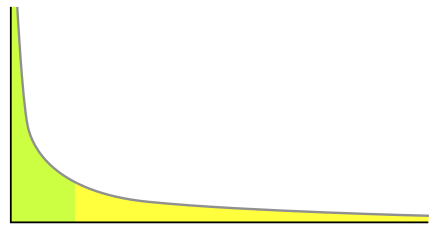
\includegraphics[height=4cm]{figure/long_tail_distribution.png}
\caption{长尾分布示意图}
\label{fig:long-tail}
\end{figure}
\subsubsection{多级反馈队列调度}
多级反馈队列(MLFQ)调度算法将就绪队列分成多个独立队列。根据进程的优先级分配到相应队列,每个队列可以有各自不同的调度算法,如前台进程和后台进程可以分成两个队列;前台进程使用RR算法,后台进程使用FCFS算法。此外,队列之间也存在调度,通常采用固定优先级抢占调度。MLFQ调度算法可以由如下五个参数定义:
\begin{itemize}
    \item 队列数量
    \item 各队列采用的调度算法
    \item 升级到较高优先级的条件
    \item 降级到较低优先级的条件
    \item 进程提交时进入某个队列的条件
\end{itemize}
MLFQ的定义使它成为CPU调度中最常采用的机制,因为它可以被配置以适应各种系统或场景。在数据中心网络中交换机对于数据流的处理可以采用MLFQ调度算法,且其较多参数的特点赋予人工智能算法以施展其强大函数拟合能力的空间。
\subsection{PIAS架构下的流量调度}

PIAS\cite{bai2015pias}默认已有较好的负载均衡算法,主要考虑数据中心网络中的流量调度问题。PIAS主要由以下三部分构成:1)中心控制器周期性地从端系统采集流量信息,计算数据流进入MLFQ各队列的阈值,并将计算结果分发至各端系统;2)端系统使用该阈值为即将发送的数据包标记优先级;3)交换机采用MLFQ调度算法将数据流继续向目的地址转发。PIAS架构的主要贡献在于解决了如下的三个问题:
\begin{itemize}
    \item 如何确定数据流进入MLFQ队列的阈值:PIAS通过遗传算法解决了FCT的最小化问题,确定了性能良好的MLFQ的阈值
    \item 数据中心的流量时刻在变化,如何保证动态环境中PIAS的表现:受到基于ECN的速率控制\cite{alizadeh2010dctcp}的启发,PIAS也采用相似的机制缓解了已确定的阈值与变化的数据流量特征间的不匹配问题。
    \item 如何保证PIAS与TCP/IP协议栈的兼容性:PIAS在端系统中采用DCTCP协议或其他包含ECN通知的其他legacy TCP协议。
\end{itemize}
\begin{figure}[ht]
\centering
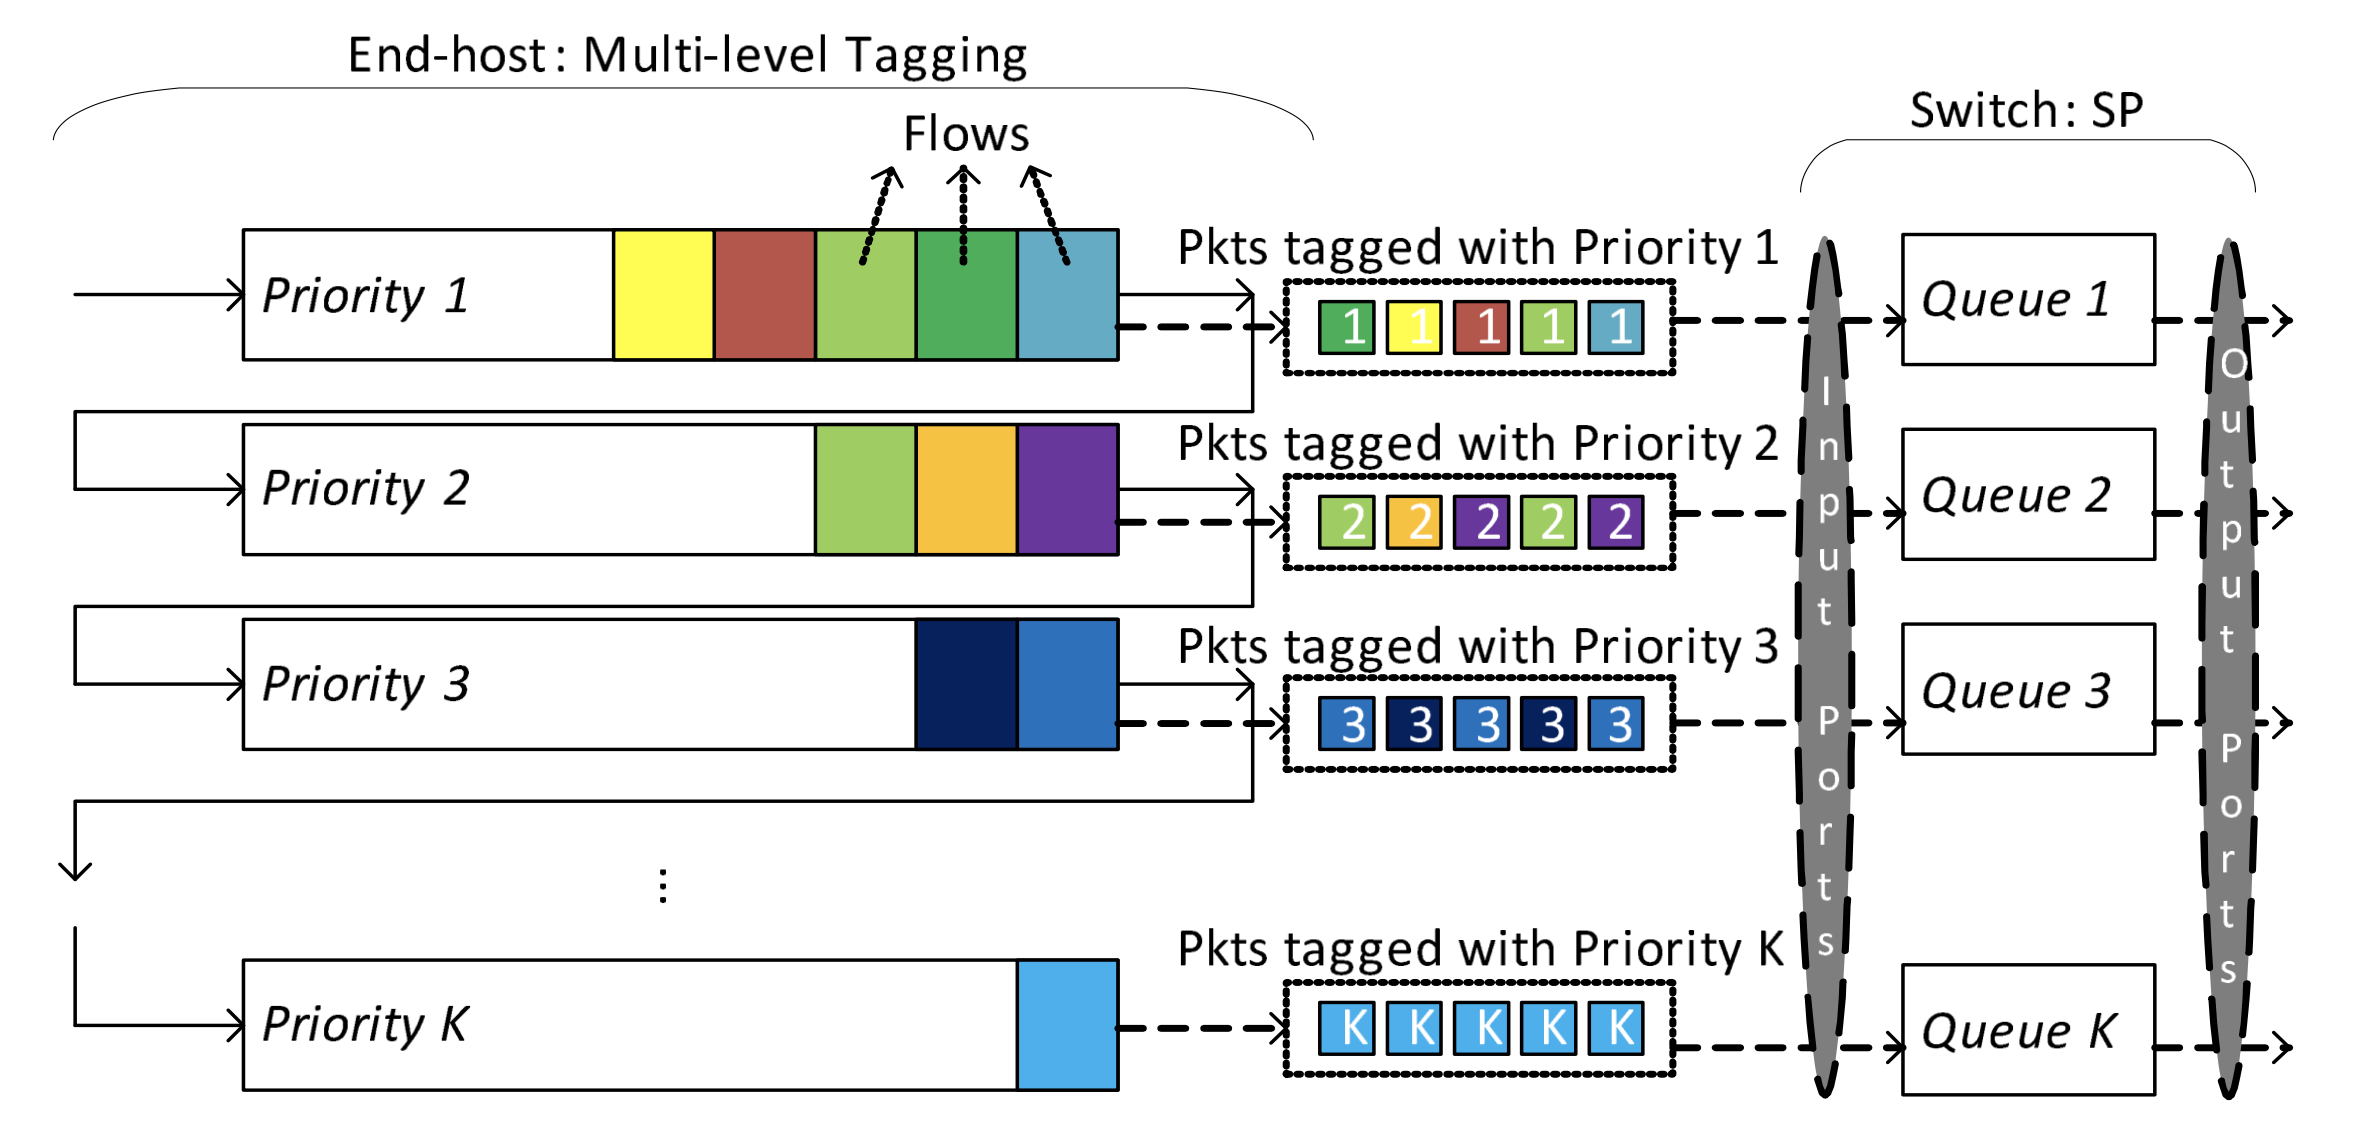
\includegraphics[height=5cm]{figure/PIAS_archi.png}
\caption{PIAS中的多级反馈队列}
\label{fig:PIAS}
\end{figure}